%% Curriculum Vitae (version 2: senior-faculty layout) -- Dr. Reetesh Kumar Gangwar
%% Single file. Compile with pdfLaTeX:  latexmk -pdf cv-v2.tex
%% Last updated: November 2026

\documentclass[11pt,a4paper]{article}

%% ---------- Page and fonts ----------
\usepackage[a4paper,left=1.9cm,right=1.9cm,top=1.6cm,bottom=1.7cm,footskip=0.9cm]{geometry}
\usepackage[T1]{fontenc}
\usepackage[p,osf,swashQ]{cochineal}
\usepackage[medium,bold]{cabin}
\usepackage[varqu,varl,scale=0.9]{zi4}
\usepackage[protrusion=true,expansion=true,tracking=true]{microtype}
\usepackage[dvipsnames]{xcolor}
\usepackage{graphicx,tabularx,longtable,array,booktabs,ragged2e}
\usepackage[fixed]{fontawesome5}
\usepackage{titlesec,enumitem,fancyhdr,lastpage,needspace}
\usepackage[colorlinks=true,allcolors=Ink,breaklinks=true]{hyperref}

%% ---------- Colours ----------
\definecolor{Ink}{HTML}{1E3550}      % headings, name
\definecolor{Accent}{HTML}{8C1D40}   % small highlights, links
\definecolor{Muted}{HTML}{5A6472}    % dates, secondary text
\definecolor{Rule}{HTML}{B9C3CF}     % hairlines
\definecolor{Tint}{HTML}{EEF2F6}     % profile box fill

\hypersetup{pdftitle={Curriculum Vitae - Dr. Reetesh Kumar Gangwar},pdfauthor={Reetesh Kumar Gangwar}}
\setlength{\parindent}{0pt}
\setlength{\parskip}{0pt}
\RaggedRight

%% ---------- Section headings ----------
\newcommand{\secfmt}[1]{\textls[60]{\MakeUppercase{#1}}}
\titleformat{\section}{\sffamily\bfseries\large\color{Ink}}{}{0pt}
  {\secfmt}[\vspace{2pt}{\color{Rule}\titlerule[0.7pt]}]
\titleformat*{\subsection}{\sffamily\bfseries\normalsize\color{Accent}}
\titlespacing*{\section}{0pt}{11pt}{5pt}
\titlespacing*{\subsection}{0pt}{7pt}{3pt}
\newcommand{\sectionnb}[1]{\section*{#1}}   % unnumbered sections

%% ---------- Footer ----------
\pagestyle{fancy}
\fancyhf{}
\renewcommand{\headrulewidth}{0pt}
\fancyfoot[L]{\footnotesize\sffamily\color{Muted}Reetesh Kumar Gangwar \textperiodcentered\ Curriculum Vitae \textperiodcentered\ November 2026}
\fancyfoot[R]{\footnotesize\sffamily\color{Muted}Page \thepage\ of \pageref{LastPage}}

%% ---------- Building blocks ----------
% Dated entry: \dated{date}{content}; content may contain \\ and \hfill
\newlength{\datew}\setlength{\datew}{2.75cm}
\newcommand{\dated}[2]{%
  \begin{list}{}{\setlength{\leftmargin}{\datew}\setlength{\labelwidth}{\datew}%
    \setlength{\labelsep}{0pt}\setlength{\topsep}{0pt}\setlength{\partopsep}{0pt}%
    \setlength{\itemsep}{0pt}\setlength{\parsep}{0pt}}
  \item[{\makebox[\datew][l]{\small\color{Muted}#1}}]#2
  \end{list}\vspace{3.5pt}}
% Second line inside a dated entry
\newcommand{\sub}[1]{\par{\small #1}}
% Role / status flags, right-aligned on the first line
\newcommand{\rs}{\kern-0.2em\scalebox{0.8}{\faRupeeSign}\kern-0.15em}
\newcommand{\amt}[1]{\textcolor{Ink}{\rs#1~lakh}}
\newcommand{\ongoing}{\textcolor{Accent}{\sffamily\small Ongoing}}
\newcommand{\done}{\textcolor{Muted}{\sffamily\small Completed}}
% Numbered publication: \pub{J1}{text}
\newlength{\publw}\setlength{\publw}{1.2em}
\newcommand{\pub}[2]{%
  \par\noindent\hangindent=\publw\hangafter=1
  \makebox[\publw][l]{\color{Accent}\small\textbullet}{\small #2}\par\vspace{3pt}}
\newcommand{\me}{\textbf{R.\,K. Gangwar}}
\newcommand{\stu}[1]{\underline{#1}}
\newcommand{\doi}[1]{\href{https://doi.org/#1}{\textcolor{Accent}{doi:#1}}}
\newcommand{\lnk}[1]{\href{#1}{\textcolor{Accent}{[link]}}}
% Profile figure tile
\newcommand{\stat}[2]{%
  \begin{minipage}[t]{0.19\linewidth}\centering
    {\sffamily\bfseries\Large\color{Ink}#1}\\[1pt]
    {\footnotesize\sffamily\color{Muted}#2}
  \end{minipage}}

\begin{document}

%% =================== HEADER ===================
\newcommand{\hl}[2]{\makebox[1.6em][c]{\color{Ink}#1}\,#2}
\begin{minipage}[t]{0.80\linewidth}
  \vspace{0pt}
  {\sffamily\bfseries\fontsize{21}{25}\selectfont\color{Ink}Dr.\ Reetesh Kumar Gangwar}\\[4pt]
  {\large Associate Professor, Department of Physics}\\[1pt]
  Indian Institute of Technology Tirupati \textperiodcentered\ {\small\color{Muted}Office AB2-313, Tirupati 517619, Andhra Pradesh, India}\\[6pt]
  {\small
  \begin{tabular}{@{}l@{\hspace{1.4em}}l@{\hspace{1.4em}}l@{}}
  \hl{\faEnvelope[regular]}{\href{mailto:reetesh@iittp.ac.in}{reetesh@iittp.ac.in}} &
  \hl{\faPhone}{+91 87725 03457} &
  \hl{\faUser}{\href{https://reeteshgangwar.github.io}{reeteshgangwar.github.io}} \\[2pt]
  \hl{\faUniversity}{\href{https://physics.iittp.ac.in/DrReetesh.html}{Institute profile}} &
  \hl{\faGlobe}{\href{https://www.ppliittp.com}{Lab: ppliittp.com}} &
  \hl{\faGraduationCap}{\href{https://scholar.google.co.in/citations?user=r6HvPAsAAAAJ}{Google Scholar}} \\[2pt]
  \hl{\faResearchgate}{\href{https://www.researchgate.net/profile/Reetesh-Gangwar-2}{ResearchGate}} &
  \hl{\faLinkedin}{\href{https://in.linkedin.com/in/plasma-processing-lab-1ab976378}{LinkedIn}} & \\
  \end{tabular}}
\end{minipage}%
\begin{minipage}[t]{0.20\linewidth}
  \vspace{0pt}\raggedleft
  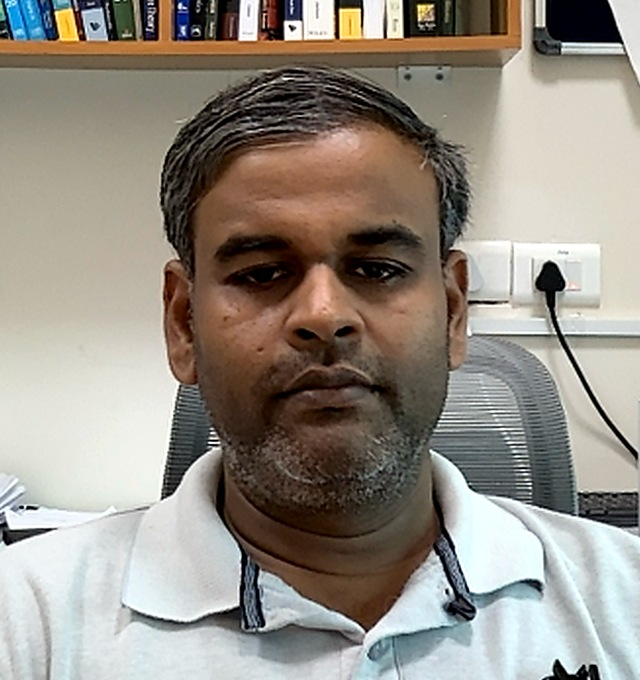
\includegraphics[width=0.92\linewidth]{photo.jpg}
\end{minipage}

\vspace{8pt}
%% =================== PROFILE AT A GLANCE ===================
\noindent\colorbox{Tint}{\begin{minipage}{\dimexpr\linewidth-2\fboxsep}
\vspace{6pt}
\stat{50+}{journal\\papers}\hfill
\stat{1,434}{citations\\h-index 18}\hfill
\stat{3\,+\,5}{Ph.D.\ students\\graduated + ongoing}\hfill
\stat{\rs3.58 Cr}{research funding\\9 projects, PI on 5}\hfill
\stat{2}{patent\\filings}
\vspace{6pt}
\end{minipage}}
{\scriptsize\color{Muted}\hfill Citation figures: Google Scholar, October 2026.}

%% =================== RESEARCH INTERESTS ===================
\sectionnb{Research Interests}
\begin{itemize}[leftmargin=1.2em,itemsep=1pt,topsep=2pt,label={\color{Accent}\small\textbullet}]
  \item Design and development of low-temperature plasma systems
  \item Optical diagnostics of plasmas and quantitative analysis of reactive species
  \item Quantum-mechanical calculation of cross sections and plasma population-kinetic modelling
  \item Classical and quantum algorithm-based plasma simulation
  \item Machine learning applications in plasma diagnostics and data analysis
  \item Plasma-based systems for water and wastewater treatment, agriculture and food processing
\end{itemize}

%% =================== EXPERIENCE ===================
\sectionnb{Professional Experience}
\dated{01/2024 -- present}{\textbf{Associate Professor}, Department of Physics, IIT Tirupati}
\dated{11/2018 -- 12/2023}{\textbf{Assistant Professor}, Department of Physics, IIT Tirupati}
\dated{03/2018 -- 11/2018}{\textbf{Assistant Professor}, Visvesvaraya National Institute of Technology (VNIT), Nagpur}
\dated{03/2016 -- 03/2018}{\textbf{Postdoctoral Researcher}, Weizmann Institute of Science, Rehovot, Israel}
\dated{11/2012 -- 03/2016}{\textbf{Postdoctoral Researcher}, Universit\'e de Montr\'eal, Montr\'eal, Canada}

%% =================== EDUCATION ===================
\sectionnb{Education}
\dated{2008 -- 2012}{\textbf{Ph.D.\ in Physics}, Indian Institute of Technology Roorkee
  \sub{Thesis: \emph{Study of collisional processes in atomic systems} (theoretical atomic and molecular physics, plasma physics)}}

%% =================== SERVICE ===================
\sectionnb{Professional Service}
\subsection*{Major administrative responsibilities at IIT Tirupati}
\dated{06/2025 -- present}{\textbf{Advisor, Outreach} (equivalent to Associate Dean)}
\dated{2025 batch}{\textbf{Faculty Advisor}, M.Sc.\ Physics}
\dated{06/2021 -- 06/2024}{\textbf{Head, Department of Physics}}
\dated{08/2019 -- 08/2021}{\textbf{Hostel Warden}}
\subsection*{Service to the scientific community}
\dated{10/2026 -- present}{\textbf{Editorial Board Member}, \emph{Plasma Sources Science and Technology} (IOP Publishing) \href{https://publishingsupport.iopscience.iop.org/journals/plasma-sources-science-and-technology/editorial-board/}{\textcolor{Accent}{[link]}}}
\dated{Editorial}{\textbf{Guest Editor}, \emph{IEEE Transactions on Plasma Science}, Special Issue on PLASMA 2025 (40th PSSI National Symposium) \href{https://ieeexplore.ieee.org/document/11349678}{\textcolor{Accent}{[link]}}}
\dated{Societies}{\textbf{Executive Board Member}, Plasma Science Society of India and Power Beam Society of India}
\dated{Conferences}{\textbf{Scientific Advisory Committee}, ISPC 2025, PLASMA 2024, PLASMA 2023 and other conferences}
\dated{Reviewing}{\textbf{Reviewer} for IEEE, Elsevier, Wiley, IOP Publishing, Springer Nature and APS journals; \textbf{examiner} for Ph.D.\ theses and project proposals}

%% =================== PROJECTS ===================
\sectionnb{Research Funding}
\subsection*{Sponsored research projects}
\dated{2026 -- 2029}{\textbf{DST, National Quantum Mission (NQM)} \hfill{\small\sffamily Co-PI \textperiodcentered\ \amt{70.64} \textperiodcentered\ }\ongoing
  \sub{\emph{Quantum machine learning: Reservoir computing and PDE solvers}}}
\dated{2025 -- 2026}{\textbf{SS Deepam Biotek Pvt.\ Ltd.} \hfill{\small\sffamily Co-PI \textperiodcentered\ \amt{25.06} \textperiodcentered\ }\ongoing
  \sub{\emph{Atmospheric nonthermal plasma-based liquid fertilizer as a natural growth enhancer and biocidal agent}}}
\dated{2024 -- 2027}{\textbf{DST-SERB, Core Research Grant} \hfill{\small\sffamily PI \textperiodcentered\ \amt{53.61} \textperiodcentered\ }\ongoing
  \sub{\emph{A novel nonthermal atmospheric pressure plasma reactor for the prevention of aflatoxin in food and agriculture products}}}
\dated{2023 -- 2028}{\textbf{DST, Centre of Excellence} \hfill{\small\sffamily Co-PI \textperiodcentered\ \amt{97.36} \textperiodcentered\ }\ongoing
  \sub{\emph{Membrane technologies for desalination, brine management and water recycling}}}
\dated{2023 -- 2026}{\textbf{DAE-BRNS} \hfill{\small\sffamily PI \textperiodcentered\ \amt{17.22} \textperiodcentered\ }\done
  \sub{\emph{An atomic processes database using calculation and measurement in tokamak and laboratory plasmas}}}
\dated{2020 -- 2021}{\textbf{DST-SERB, Special Call on COVID-19} \hfill{\small\sffamily PI \textperiodcentered\ \amt{20.10} \textperiodcentered\ }\done
  \sub{\emph{A portable optical cavity sterilization unit}}}
\dated{2019 -- 2022}{\textbf{DST-SERB, Core Research Grant} \hfill{\small\sffamily PI \textperiodcentered\ \amt{24.45} \textperiodcentered\ }\done
  \sub{\emph{A novel scheme to cool the translational and internal degrees of freedom of any molecular ion beam}}}
\subsection*{Industry consultancy}
\dated{2025}{\textbf{FaradayEarth Pvt.\ Ltd.} \hfill{\small\sffamily PI \textperiodcentered\ \amt{2.36} \textperiodcentered\ }\done
  \sub{\emph{Optical diagnostics of an industry preparatory atmospheric-pressure plasma reactor and feasibility of ML-based optical diagnostics}}}
\dated{2024 -- 2025}{\textbf{Ozone Research and Applications India Pvt.\ Ltd.} \hfill{\small\sffamily Co-PI \textperiodcentered\ \amt{47.59} \textperiodcentered\ }\done
  \sub{\emph{Atmospheric nonthermal plasma-based liquid fertilizer as a natural growth enhancer and biocidal agent}}}

%% =================== PUBLICATIONS ===================
\sectionnb{Publications, 2024 -- 2026}
{\small\color{Muted}\textbf{Bold}: R.\,K. Gangwar. \underline{Underlined}: students and postdoctoral fellows supervised. Complete list on
\href{https://scholar.google.co.in/citations?user=r6HvPAsAAAAJ&hl=en}{\textcolor{Accent}{Google Scholar}}.}

\subsection*{Under review}
\pub{P2}{\stu{K. Paul}, R. V, S. Aravinda and \me, ``Efficient quantum simulation of linearized Vlasov--Poisson dynamics using Trotter and THRIFT Hamiltonian simulation methods'', arXiv:2608.23127 (2026). \lnk{https://arxiv.org/abs/2608.23127}}
\pub{P1}{\stu{R. Dey}, A. Agarwal, \me, D. Sharma, M.\,B. Chowdhuri, R. Srivastava and J. Ghosh, ``Relativistic calculations of electron impact excitation cross-sections of neutral tungsten'', arXiv:2603.02612 (2026). \lnk{https://arxiv.org/abs/2603.02612}}

\subsection*{Journal articles -- 2026}
\pub{J19}{\stu{T. Pushparaj Gandhi}, Somya Pal, Sriramulu Maniteja, \me\ and Shihabudheen M. Maliyekkal, ``Synergistic falling film nonthermal plasma and UV-photon hybrid system: An advanced and energy-efficient approach for rapid dye degradation'', \emph{Separation and Purification Technology} (2026). \doi{10.1016/j.seppur.2026.140781}}
\pub{J18}{\stu{S.\,B. Thota}, \stu{P.\,S.\,N.\,S.\,R. Srikar}, \stu{S. Mathengattil}, S.\,M. Maliyekkal and \me, ``Phase-resolved optical diagnostics of waveform-modulated Ar nonthermal atmospheric pressure plasma jet'', \emph{Spectrochim.\ Acta B}, 107649 (2026). \lnk{https://www.sciencedirect.com/science/article/pii/S0584854726002004}}
\pub{J17}{\stu{M.\,G.\,B. Narayana}, \stu{I. Suresh} and \me, ``Calculation of fine structure resolved electron impact excitation cross sections of Al I using relativistic distorted wave method'', \emph{IEEE Trans.\ Plasma Sci.} (2026). \lnk{https://ieeexplore.ieee.org/abstract/document/11644741/}}
\pub{J16}{\stu{R. Dey}, \stu{I. Suresh}, D. Sharma, M.\,B. Chowdhuri, \emph{et al.}, R. Srivastava, J. Ghosh and \me, ``Fine-structure resolved electron impact excitation of O IV and O V: A comprehensive relativistic study for plasma modeling and diagnostics'', \emph{J.\ Phys.\ B: At.\ Mol.\ Opt.\ Phys.}\ \textbf{59} (14) (2026). \doi{10.1088/1361-6455/ae872a}}
\pub{J15}{A. Jayanarasimhan, A.\,U. Shetty, D. Dhanabal, S. Acharya, K.\,V.\,S.\,S. Bhargavi, \me, D. Saha and S. Ranjan, ``Warm non-equilibrium plasma-assisted catalysis for sustainable ammonia synthesis'', \emph{Green Chem.}\ \textbf{28}, 8757--8765 (2026). \lnk{https://pubs.rsc.org/gc/article-abstract/28/21/8757/1226472}}
\pub{J14}{V. Bende, \stu{P.\,S.\,N.\,S.\,R. Srikar}, \me, R.\,L. Bhardwaj and R. Kar, ``A semi-empirical approach to Boltzmann plot analysis for cold atmospheric pressure plasma: Comparison with collision-radiative modelling'', \emph{Vacuum}, 115263 (2026). \doi{10.1016/j.vacuum.2026.115263}}
\pub{J13}{\stu{R. Dey}, A. Agrawal, \me, D. Sharma, R. Srivastava, M.\,B. Chowdhuri and J. Ghosh, ``Simulation study of neutral tungsten emissions for fusion applications'', \emph{Plasma Fusion Res.}\ \textbf{21}, 2403022 (2026). \doi{10.1585/pfr.21.2403022}}
\subsection*{Journal articles -- 2025}
\pub{J12}{\stu{P.\,S.\,N.\,S.\,R. Srikar}, \stu{I. Suresh} and \me, ``Machine learning-enabled prediction of optical emission spectra in scalable non-thermal Ar atmospheric pressure plasma multi jet'', \emph{J.\ Phys.\ D: Appl.\ Phys.}\ \textbf{58}, 415204 (2025). \doi{10.1088/1361-6463/ae0b81}}
\pub{J11}{\stu{T. Pushparaj Gandhi}, M.\,G.\,C. Pavan Sai, \stu{S.\,M. Allabakshi}, \me\ and S.\,M. Maliyekkal, ``Transforming antibiotic treatment: Unleashing the nexus between UV photons and nonthermal atmospheric pressure air plasma in pharmaceutical wastewater'', \emph{J.\ Environ.\ Chem.\ Eng.}\ \textbf{13}, 119160 (2025). \lnk{https://www.sciencedirect.com/science/article/pii/S2213343725038564}}
\pub{J10}{V. Bende, V. Nagar, \stu{P.\,S.\,N.\,S.\,R. Srikar}, \me, D. Bhale, R.\,L. Bhardwaj and R. Kar, ``Reactive species dynamics and bactericidal mechanisms in cold atmospheric pressure plasma with gas admixtures'', \emph{Vacuum} \textbf{239}, 114393 (2025). \lnk{https://www.sciencedirect.com/science/article/pii/S0042207X25003835}}
\pub{J9}{\stu{T. Pushparaj Gandhi}, \stu{P.\,S.\,N.\,S.\,R. Srikar}, \stu{S.\,M. Allabakshi}, \me\ and S.\,M. Maliyekkal, ``Removal of aflatoxin B1 from solid and liquid matrices using cold atmospheric plasma reactors: Insights into reactor configurations and food quality testing'', \emph{Innov.\ Food Sci.\ Emerg.\ Technol.}, 104203 (2025). \lnk{https://www.sciencedirect.com/science/article/pii/S1466856425002875}}
\pub{J8}{P. Kumar, \stu{P.\,S.\,N.\,S.\,R. Srikar}, D. Dahatonde, \me\ and T. Nallamilli, ``Effect of atmospheric pressure cold plasma treatment on charge, structure, thermal properties and coacervation behavior of pea protein isolate with alginate'', \emph{Innov.\ Food Sci.\ Emerg.\ Technol.}\ \textbf{101}, 103948 (2025). \lnk{https://www.sciencedirect.com/science/article/pii/S1466856425000323}}
\subsection*{Journal articles -- 2024}
\pub{J7}{\stu{S.\,M. Allabakshi}, \stu{P.\,S.\,N.\,S.\,R. Srikar}, S. Gomosta, \me\ and S.\,M. Maliyekkal, ``Treatment of textile dyes in a photo-surface dielectric barrier discharge hybrid reactor: Unraveling the degradation mechanisms'', \emph{Chemosphere} \textbf{368}, 143775 (2024). \lnk{https://www.sciencedirect.com/science/article/pii/S0045653524026766}}
\pub{J6}{\stu{I. Suresh}, \stu{P.\,S.\,N.\,S.\,R. Srikar} and \me, ``Integration of ML methods with CR model-based optical diagnostic for the estimation of electron temperature in Ga laser produced plasma'', \emph{Phys.\ Plasmas} \textbf{31}, 113501 (2024). \lnk{https://pubs.aip.org/aip/pop/article/31/11/113501/3319199}}
\pub{J5}{\stu{P.\,S.\,N.\,S.\,R. Srikar}, \stu{S.\,M. Allabakshi}, S. Gomosta, S.\,M. Maliyekkal and \me, ``Development of efficient nonthermal atmospheric-pressure Ar-plasma jet through simultaneous spectroscopic characterization and radical quantification'', \emph{J.\ Phys.\ D: Appl.\ Phys.}\ \textbf{57}, 395204 (2024). \doi{10.1088/1361-6463/ad5c76}}
\pub{J4}{\stu{P.\,S.\,N.\,S.\,R. Srikar}, \stu{I. Suresh} and \me, ``Accelerated real-time plasma diagnostics: Integrating argon collisional-radiative model with machine learning methods'', \emph{Spectrochim.\ Acta B} \textbf{215}, 106909 (2024). \lnk{https://www.sciencedirect.com/science/article/pii/S0584854724000533}}
\pub{J3}{\stu{S.\,A.\,A. Balkhi}, \stu{S.\,M. Allabakshi}, \stu{P.\,S.\,N.\,S.\,R. Srikar}, S. Gomosta, \me\ and S.\,M. Maliyekkal, ``Unwinding the correlation between atmospheric pressure plasma jet operating parameters and variation in antibiotic wastewater characteristics'', \emph{J.\ Water Process Eng.}\ \textbf{60}, 105186 (2024). \lnk{https://www.sciencedirect.com/science/article/pii/S2214714424004185}}
\pub{J2}{\stu{I. Suresh}, R. Srivastava and \me, ``Fully relativistic distorted wave calculations of electron impact excitation of gallium atom: Cross sections relevant for plasma kinetic modeling'', \emph{Spectrochim.\ Acta B} \textbf{213}, 106860 (2024). \lnk{https://www.sciencedirect.com/science/article/pii/S0584854724000041}}
\pub{J1}{\stu{I. Suresh}, Priti, R. Srivastava and \me, ``Fine structure resolved excitation cross sections of singly ionized Ga for the modeling and diagnostics of Ga plasmas'', \emph{Plasma Sources Sci.\ Technol.}\ \textbf{33}, 025018 (2024). \doi{10.1088/1361-6595/ad27ec}}

\subsection*{Book chapter -- 2025}
\pub{B1}{\stu{S.\,M. Allabakshi}, \stu{P.\,S.\,N.\,S.\,R. Srikar}, \me\ and S.\,M. Maliyekkal, ``Nonthermal plasma technology for degradation of dyes in wastewater'', in \emph{Innovative and Hybrid Advanced Oxidation Processes for Water Treatment}, Elsevier, pp.\ 255--278 (2025). \lnk{https://www.sciencedirect.com/science/article/pii/B9780443141003000016}}

\subsection*{Patents}
\pub{IP2}{S.\,M. Maliyekkal, \me, \stu{S.\,M. Allabakshi}, \stu{P.\,S.\,N.\,S.\,R. Srikar} and \stu{A. Kumar}, ``Chemo-photo-plasma hybrid advanced oxidation process for ultrafast removal of environmental pollution'' \textcolor{Muted}{(invention disclosure submitted)}}
\pub{IP1}{S.\,M. Maliyekkal, S. Soujit, G. Vajitha, \stu{P.\,S.\,N.\,S.\,R. Srikar} and \me, ``Plasma-UV assisted bulk production of graphenic material with tunable surface area and porosity'' \textcolor{Muted}{(complete patent application filed)}}

%% =================== TEACHING ===================
\needspace{10\baselineskip}
\sectionnb{Teaching at IIT Tirupati}
{\small
\renewcommand{\arraystretch}{1.08}
\setlength{\LTpre}{0pt}\setlength{\LTpost}{0pt}
\begin{longtable}{@{}>{\leavevmode\sffamily\color{Muted}}p{2.45cm} >{\RaggedRight\arraybackslash}p{5.6cm} >{\RaggedRight\arraybackslash}p{\dimexpr\linewidth-8.05cm-4\tabcolsep\relax}@{}}
\toprule
\textbf{\color{Ink}Code} & \textbf{Course} & \textbf{Semesters taught (latest first)} \\
\midrule
\endfirsthead
\toprule
\textbf{\color{Ink}Code} & \textbf{Course} & \textbf{Semesters taught (continued)} \\
\midrule
\endhead
\multicolumn{3}{@{}l}{\sffamily\bfseries\color{Accent}Undergraduate} \\
PH301P & Applied Optics and Material Physics Laboratory & Jul--Dec 2026 \\
PH105L & Introduction to Quantum Science and Technology & Jul--Dec 2026, 2025, 2024 \\
PH001L & Physics Preparatory Course & Jul--Dec 2023 \\
PH1103 / PH103P & Physics Laboratory & Jul--Dec 2025, 2022, 2019 \textperiodcentered\ Jan--Jun 2024, 2023, 2021, 2020, 2019 \textperiodcentered\ Summer 2023, 2022 \\
PH1202 & Introduction to Electrodynamics and Quantum Mechanics & Jan--Jun 2020, 2019 \\
PH1101 & Introduction to Classical Mechanics & Jul--Dec 2019 \\[2pt]
\multicolumn{3}{@{}l}{\sffamily\bfseries\color{Accent}Postgraduate and Ph.D.} \\
PH605L & Basics and Applications of Plasma Physics & Jul--Dec 2026, 2025, 2024, 2021, 2020, 2019 \textperiodcentered\ Jan--Jun 2024, 2023, 2022 \\
PH511L & Quantum Mechanics II & Jan--Jun 2026, 2025 \\
PH507L & Mathematical Physics II & Jan--Jun 2024, 2023, 2022, 2021 \\
PH702L & Foundations of Experimental Physics & Jan--Jun 2024, 2023, 2022 \\
PH603P & Advanced Physics Laboratory & Jul--Dec 2024, 2023 \\
PH508P & Physics Laboratory I & Jul--Dec 2024, 2023 \\
PH691G & Project Phase I & Every Jul--Dec semester, 2021 -- present \\
PH692G & Project Phase II & Every Jan--Jun semester, 2022 -- present \\
\bottomrule
\end{longtable}}

%% =================== SUPERVISION ===================
\sectionnb{Research Supervision}
\subsection*{Ph.D.\ graduates (3)}
\dated{2020 -- 2025}{\textbf{Dr.\ Indhu Suresh} \hfill{\small\color{Muted}now Postdoctoral Researcher, ITER-India}
  \sub{\emph{Relativistic calculation of cross sections for electron-induced processes and their application in optical plasma diagnostics and machine learning methods}}}
\dated{2019 -- 2025}{\textbf{Dr.\ P.\,S.\,N.\,S.\,R. Srikar} \hfill{\small\color{Muted}now Plasma--Neutral Interactions Physicist, UKAEA}
  \sub{\emph{Characterization and application of atmospheric pressure plasmas by integrating optical spectroscopy with generalized population-kinetic models and machine learning methods}}}
\dated{2019 -- 2024}{\textbf{Dr.\ S.\,M. Allabakshi} {\small(joint, with Dr.\ S.\,M. Maliyekkal)} \hfill{\small\color{Muted}now Postdoctoral Scientist, CAES, USA}
  \sub{\emph{Development of a novel nonthermal atmospheric pressure photo-plasma reactor for efficient treatment of textile wastewater}}}

\subsection*{Ph.D.\ scholars, ongoing (5)}
\dated{2024 -- present}{\textbf{Mr.\ Shriyash Vilas Patil} -- \emph{Machine learning in plasma diagnostics}}
\dated{2024 -- present}{\textbf{Mr.\ M. Guru Bhavan Narayana} -- \emph{Machine learning in plasma modelling and diagnostics}}
\dated{2024 -- present}{\textbf{Mr.\ Abhay Kumar} -- \emph{Plasma-based wastewater treatment} {\small(joint)}}
\dated{2022 -- present}{\textbf{Mr.\ T. Satish Babu} -- \emph{Plasma-assisted synthesis and alteration of materials} {\small(joint)}}
\dated{2022 -- present}{\textbf{Mr.\ T. Pushparaj Gandhi} -- \emph{Plasma treatment of mycotoxin-contaminated food} {\small(joint)}}
{\footnotesize\color{Muted}Joint supervision with Dr.\ Shihabudheen M.\ Maliyekkal, IIT Tirupati.}

\subsection*{Postdoctoral fellow}
\dated{}{\textbf{Dr.\ Ritu Dey} -- \emph{Cross-section calculations using relativistic distorted-wave (RDW) theory}}

\subsection*{M.S.\ (Research)}
\dated{}{\textbf{Ms.\ Akhila K.\,C.} (IISER Tirupati)}

\subsection*{Master's and project students}
{\small
\renewcommand{\arraystretch}{1.12}
\begin{tabularx}{\linewidth}{@{\hspace{\datew}}X X@{}}
\textbf{\sffamily\color{Ink}M.Tech.\ / M.S.\ / Project} & \textbf{\sffamily\color{Ink}M.Sc.} \\[1pt]
Ms.\ Shanila M.\ (Project)          & Mr.\ Kartik Paul \\
Ms.\ Somya Pal (M.Tech.)            & Mr.\ Diwaskar Rai \\
Mr.\ Rahul Kumar (M.Tech.)          & Mr.\ Akash Uniyal \\
Ms.\ Priyanshi Chauhan (Project)    & Ms.\ Anamika \\
Mr.\ Jerin Abraham George (M.S.)    & Ms.\ Chebrolu Rajyalakshi \\
Ms.\ Syed Arwa Balkhi (M.Tech.)     & Mr.\ Debabrat Rout \\
Ms.\ Palli Priyanka (M.Tech.)       & Ms.\ Saroj Meena \\
                                    & Ms.\ Sajal Soan \\
                                    & Ms.\ Muskan \\
                                    & Mr.\ Amit Kumar Jangid \\
                                    & Mr.\ Rahul Samriya \\
\end{tabularx}}

%% =================== TALKS ===================
\sectionnb{Invited Talks and Outreach}
\dated{Apr 2026}{\textbf{Keynote}: \emph{Atmospheric pressure plasma: A sustainable platform for next-generation technologies}, Int.\ Conf.\ on Advanced Functional Materials \& Quantum Science for Sustainable \& Smart Technologies, KL University}
\dated{Dec 2025}{\emph{Feasibility of data-driven approaches in optical diagnostics of non-equilibrium plasmas}, 2nd National Symposium on Gaseous Discharges (NSGD-2025), Pondicherry University}
\dated{Sep 2025}{\emph{Optimization of reactive species generation in nonthermal atmospheric pressure Ar plasma using machine learning}, 9th Asia-Pacific Conference on Plasma Physics}
\dated{May 2025}{\emph{Smart diagnostics of nonthermal atmospheric pressure plasmas for efficient reactor development}, IIT Mandi}
\dated{Mar 2026}{FDP: \emph{Quantum superposition and entanglement in search and communication algorithms}, Sri Venkateswara University, Tirupati}
\dated{Dec 2025}{FDP: \emph{Quantum playbook: From superpositions to entanglements and beyond}, Siddhartha Institute of Science and Technology, Puttur}
\dated{Sep 2025}{ATAL FDP: \emph{Basics and applications of plasma physics}, Ashoka Women's Engineering College, Kurnool}

%% =================== HONOURS ===================
\sectionnb{Fellowships and Honours}
\dated{2018}{\textbf{Dean of Faculty Fellowship}, Weizmann Institute of Science, Israel}
\dated{2014}{\textbf{Visiting Researcher}, PROMES-CNRS, Perpignan, France}
\dated{2010}{\textbf{Commonwealth Exchange Program (Asia-Pacific) Research Grant}, DFAIT Canada, for collaboration with Prof.\ A.\,D. Stauffer, York University, Toronto}
\dated{July, 2007}{\textbf{CSIR-NET Junior and Senior Research Fellowships} (Physical Sciences)}

%% =================== MEMBERSHIPS ===================
\sectionnb{Memberships}
\begin{itemize}[leftmargin=1.2em,itemsep=1pt,topsep=2pt,label={\color{Accent}\small\textbullet}]
  \item Life Member, Indian Society of Atomic and Molecular Physics (ISAMP), No.\ 1371
  \item Life Member, Indian Physics Association (IPA), No.\ ROO/LM/12792
  \item Life Member, Plasma Science Society of India (PSSI), No.\ LM 906
  \item Life Member, Power Beam Society of India (PBSI), No.\ 105
  \item Life Member, Division of Plasma Physics, Association of Asia Pacific Physical Societies (AAPPS-DPP), No.\ 2997
\end{itemize}

\end{document}
